La caracterización de las propiedades de los muones es parte importante de este estudio, obtener las dependencias empíricas entre ellas y los posibles cambios en los límites de estas propiedades resultado del cambio de la eficiencia de los detectores en sus diferentes configuraciones se hace necesario para comprender mejor como se visualiza la teoría investigada desde su reconstrucción por los detectores.

Dado la necesidad de hacer referencia a las propiedades de los muones se hará uso de la variable $\chi$, esta puede ocupar las variables: 

%\begin{tabular}{p{2.5cm}p{11.5cm}}
\begin{itemize_f}
\item[-] \texttt{\textbf{P}}: momento de la partícula, normalmente referenciada por su proyección en dirección transversal \texttt{\textbf{PZ}} $=$ \texttt{\textbf{P}} $\sin \theta$, donde $\theta$ es el ángulo polar, definido como aquel entre el vector momento y la dirección positiva del as, normalmente utilizado ya que no es invariante frente a transformaciones de Lorentz.\\
\item[-] $\mathbf{\eta}$: la pseudoapidez (también referida como \texttt{Eta}), esta representa la coordenada espacial que describe el ángulo de una partícula en relación con el eje del haz. Su ecuación tiene la forma:
\begin{equation}
\eta = -\ln \left[ \tan \left( \dfrac{\theta}{2} \right)\right]
\end{equation}

\item[-] $\mathtt{\phi}$: ángulo azimutal (también referida como \texttt{Phi}).\\
\item[-] \textbf{\texttt{T}} tiempo de vida media, esta describe la descomposición de las partículas, se expresa comúnmente en términos de vida media, constante de descomposición o vida media. La probabilidad de descomposición se puede expresar como una función de distribución:
\begin{equation}
W (t)~ = ~ A e^{-\lambda t} 
\end{equation}
Para normalizar esta función de distribución:
\begin{equation}
\int_0^\infty W (t) dt ~ = ~ \int_0^\infty A e^{-\lambda t} dt = ~ - \left. \dfrac{1}{\lambda} A e^{-\lambda t} \right|_0^\infty = \dfrac{A}{\lambda} = 1
\end{equation}
La probabilidad de que una partícula dada decaiga dentro del tiempo $t$ viene dada por la integral de la función de distribución de descomposición de $0$ a $t$. Esta no es la cantidad que deseamos calcular: queremos el tiempo promedio que la partícula existirá sin descomponerse. La probabilidad de que una partícula no se descomponga es uno menos la probabilidad de que se descomponga. La probabilidad de que una partícula permanezca en el tiempo $t$ es entonces:
\begin{equation}
P_W(t) ~ = ~ 1 - \int_0^t \lambda e^{-\lambda t'} dt' ~ = ~ 1 +  \left. e^{-\lambda t'} \right|_0^t = e^{-\lambda t}
\end{equation}
El tiempo de supervivencia promedio es entonces el valor medio del tiempo usando esta función de probabilidad tenemos.
\begin{equation}
<t>~ = ~ \tau ~ = ~ \int_0^t te^{-\lambda t} dt/\int_0^t e^{-\lambda t} dt = \lambda \int_0^\infty e^{-\lambda t} dt ~ = \dfrac{1}{\lambda}
\end{equation}

\item[-] \texttt{D0}: Parámetro de impacto transversal, se define como la distancia transversal al eje del haz en el punto de maxima aproximacion, donde su signo esta dado de acuerdo al momento angular de la traza alrededor de eje.\\

\item[-] \texttt{DZ}: Parámetro de impacto longitudinal, definido como la posicion de la coordenada $z$ de la traza en el punto de maximo acercamiento.\\
%\item[-] \texttt{IsolationVar} xxx\\
%\item[-] \texttt{SumPt} xxx\\
%\item[-] \texttt{SumPtNeutral}: xxx\\
%\item[-] \texttt{SumPtCharged}: xxx\\
%\item[-] \texttt{IsolationVar}: xxx\\
\end{itemize_f}
%\end{tabular}

Ante la necesidad de hacer estadística con las variables $\chi$ definimos la frecuencia de cada una de estas variables $\mathbb{F}_\chi^{(\mathtt{k})}$(x) donde para un valor predefinido de resolución de la información $\delta \chi$
\begin{equation}
\mathtt{\Theta(X,~Y)} ~ = ~ \Bigg\{\begin{matrix}
1 & \mathtt{X-\Delta X ~<~Y ~and~Y~ < X+\Delta X}\\
0 & \mathtt{X-\Delta X ~>~Y ~~or~~Y~ > X+\Delta X}
\end{matrix} 
\end{equation}

\begin{equation}
\mathbb{F}_\chi^{(\mathtt{k})} (x)= \sum_{ji} \mathtt{\Theta}(\chi_i^{(j,k)},~x)
\end{equation}

\begin{equation}
f_\chi^{(\mathtt{k})} (x)= \mathbb{F}_\chi^{(\mathtt{k})} (x)/ \sum_x \mathbb{F}_\chi^{(\mathtt{k})} (x)
\end{equation}


%\texttt{MNeuL}, \texttt{MNeuD}, \texttt{MPhoD}, \texttt{TcPhoD})

\subsubsection{Momento transversal.}
En los gráficos superiores de la Fig. \ref{procesos_darksusy_PTyISO} se puede observar los valores de momento angular de todos los muones reconstruidos para eventos $\mathbb{E}_i^{(4\mu,~\mathtt{CMS})}$ (configuración \texttt{Run-2}) y $\mathbb{E}_i^{(4\mu,~\mathtt{HL})}$ (configuración en \texttt{High Luminosity}), en estos se puede visualizar las diferencias entre los rangos de detección donde para eventos $k=$\texttt{CMS} el $\backsim ~ 99\%$ de los muones poseen $\sim 10  < ~ P_t^{(4\mu,~\mathtt{CMS})} ~ <\sim 100$, en contraste para $k=$\texttt{HL} tenemos $\sim 0.1 < ~ P_t^{(4\mu,~\mathtt{HL})} ~ < \sim 100$. Este aumento de rango en \texttt{HL} para valores menores de $\backsim ~ 10~GeV$ se puede ver que no es sin pérdidas, se puede constatar un cambio en la forma de los gráficos, esto es debido a que la inclusión de nuevos sensores en la configuración \texttt{HL} no poseen la misma eficiencia en la reconstrucción de la información.

\begin{figure}[h]
\centering
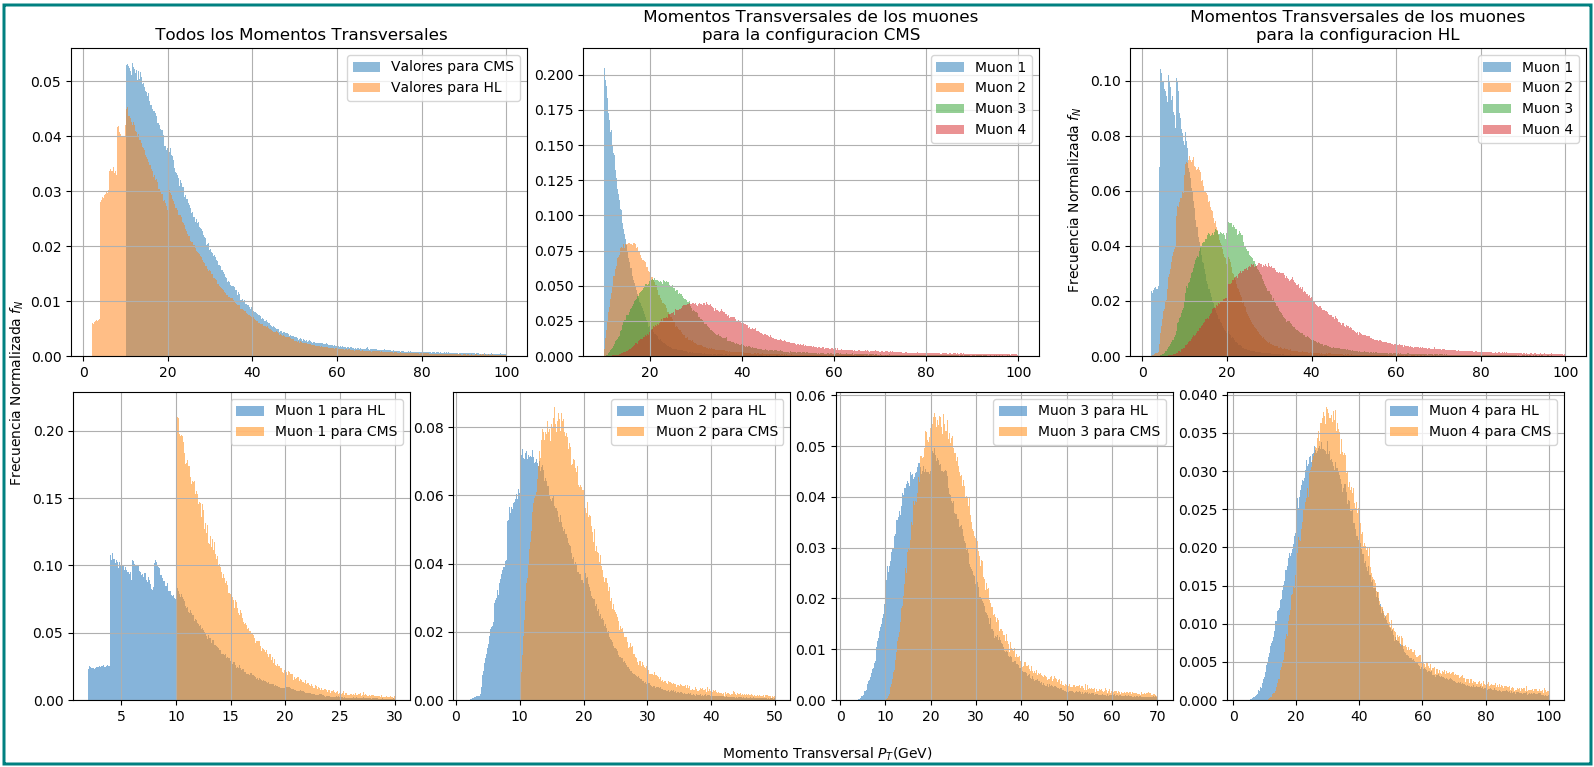
\includegraphics[width=.8\textwidth]{Simulacion/imagenes/Datos_PT_ALL.png}
%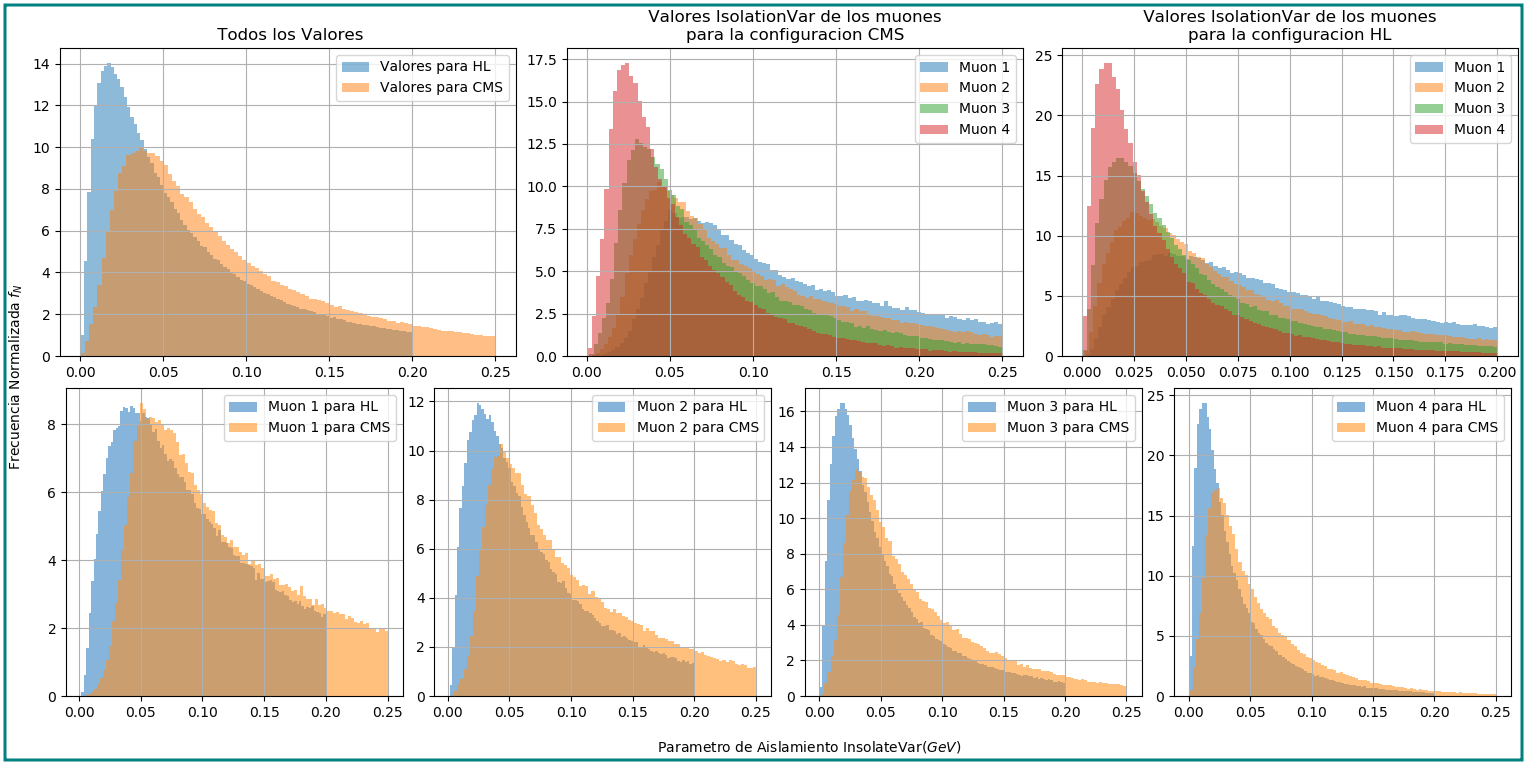
\includegraphics[width=.8\textwidth]{Simulacion/imagenes/Datos_IsolationVar_ALL.png}
\caption{Caracterización global de los momentos transversales de nuestra población de muones reconstruidos.}
\label{procesos_darksusy_PTyISO}
\end{figure}



\subsubsection{Valores de angulo}
\begin{figure}[h]
\centering
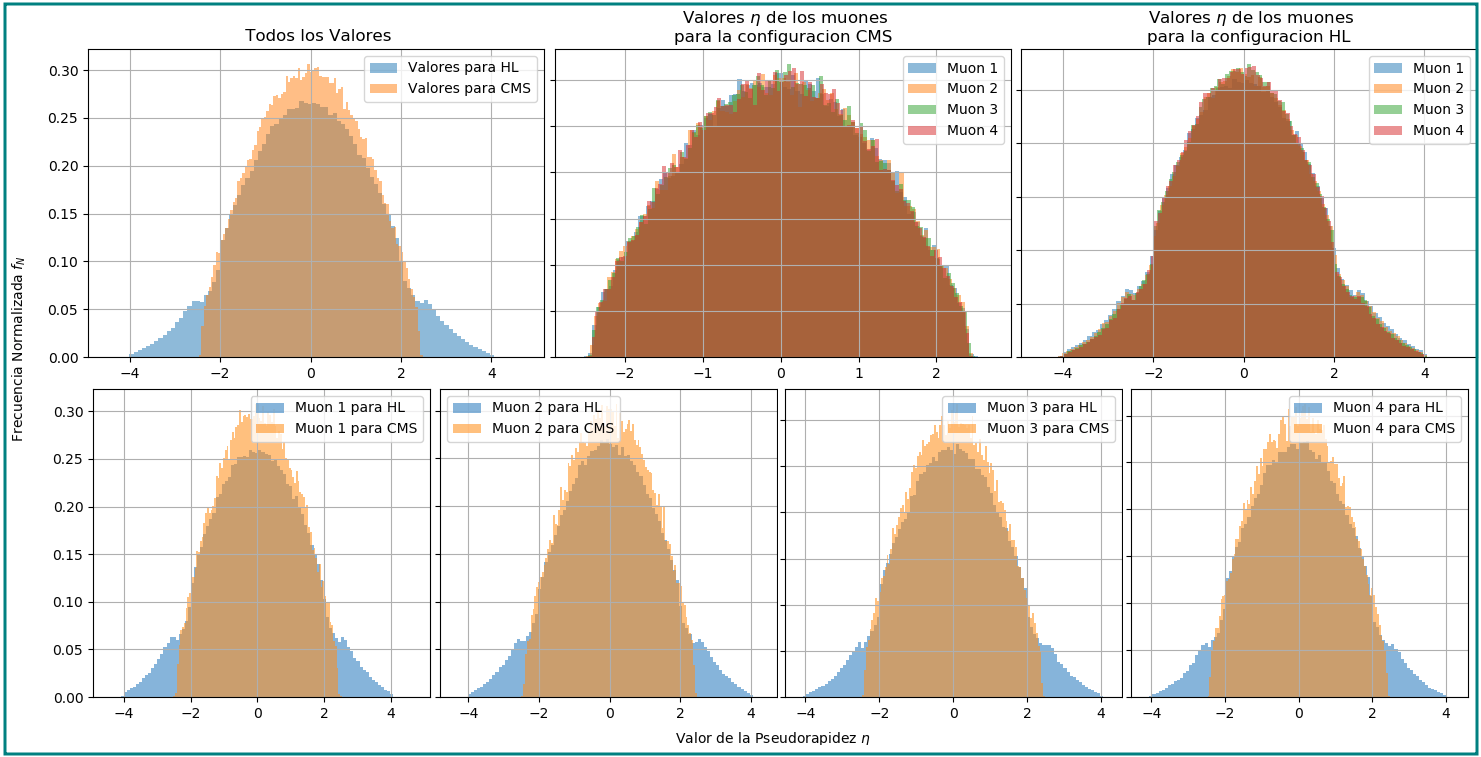
\includegraphics[width=.8\textwidth]{Simulacion/imagenes/Datos_Eta_ALL.png}
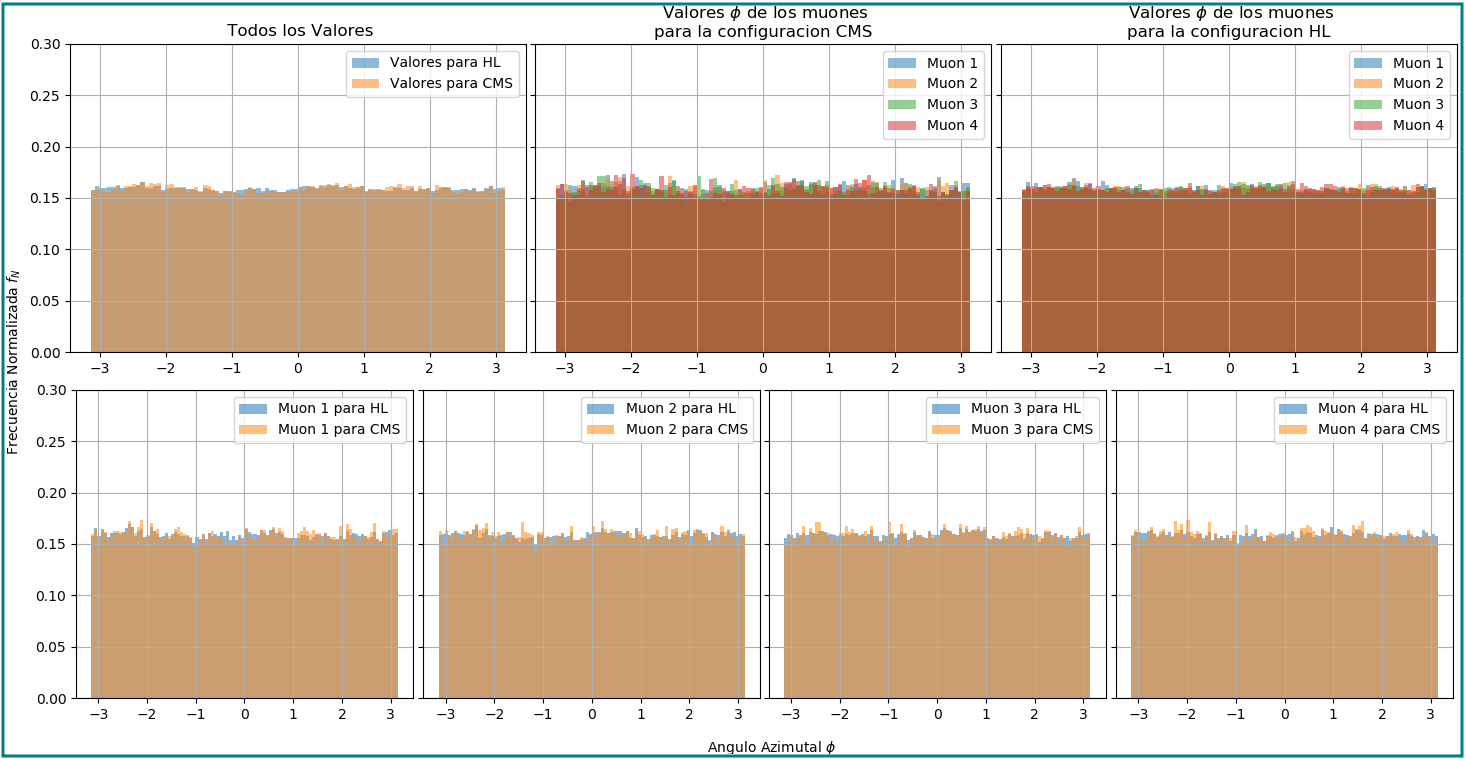
\includegraphics[width=.8\textwidth]{Simulacion/imagenes/Datos_Phi_ALL.png}
\caption{Grupo total de datos generados para los eventos de interes.}
\label{procesos_darksusy_ETAyPHI}
\end{figure}





Otro factor importante en la detección de los muones es el valor de Entonces de forma generar se puede Además como límite superior se puede constatar que el  se encuentran para valores 



















